\clearpage
\section*{Appendix}

\vspace{5cm}

\begin{figure}[h!]
  \centering
     \subfloat[$\epsilon \in \{ 10^{-1},10^{-2},10^{-3},10^{-4},10^{-5},10^{-6} \}$.]{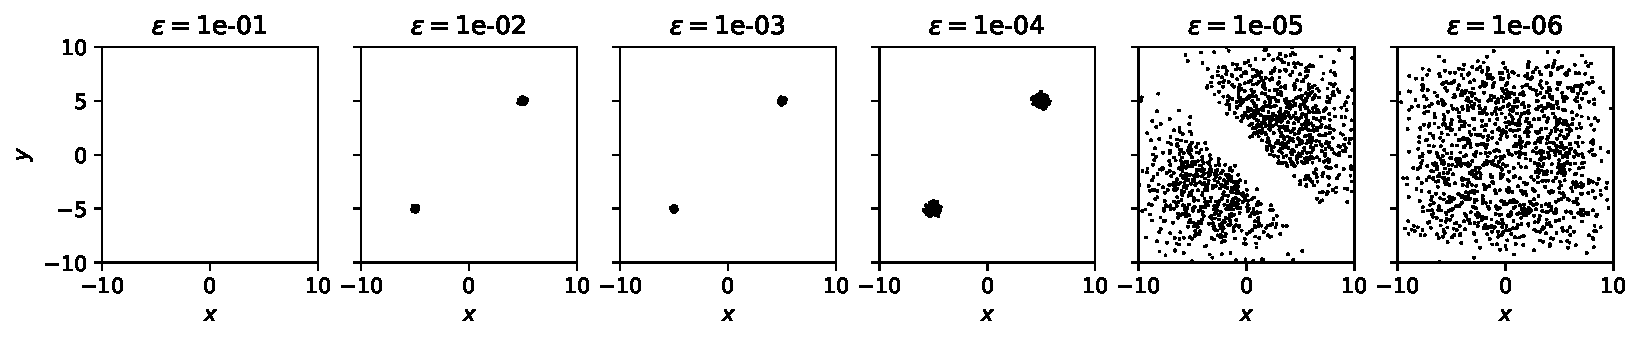
\includegraphics[width=\linewidth]{figures/toy/samples_eps_1.pdf}}\\
     \subfloat[$\epsilon \in \{ 10^{-4},8 \cdot 10^{-5},6 \cdot 10^{-5},4 \cdot 10^{-5},2 \cdot 10^{-5}, 10^{-5} \}$.]{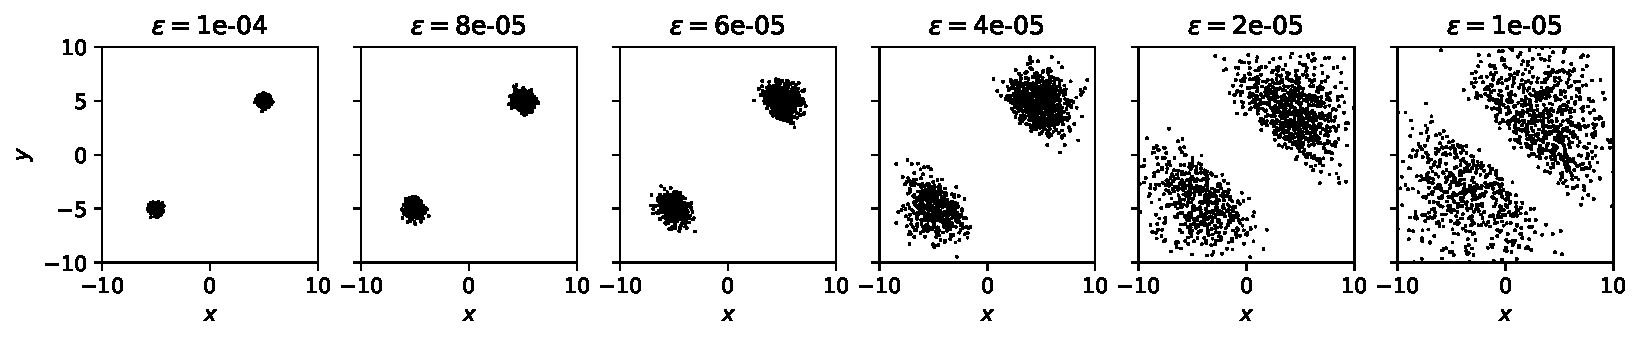
\includegraphics[width=\linewidth]{figures/toy/samples_eps_2.pdf}}
     \caption{Samples obtained with different values of $\epsilon$ for toy data with annealed Langevin dynamics. Even after expanding the search in the promising interval $\epsilon \in \{10^{-4}, 10^{-5}\}$, we did not find a value of $\epsilon$ yielding satisfying results.}
     \label{fig:eps}
\end{figure}


% \vspace{1cm}
\newpage


\begin{figure}[h!]
    \centering
    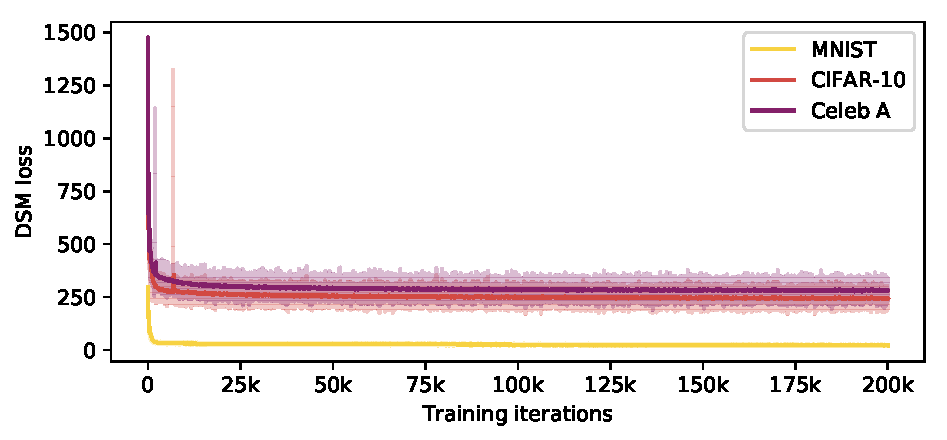
\includegraphics[width=0.90\linewidth]{figures/loss_real.pdf}
    \caption{Loss curves for training real model}
    \label{fig:losses}
\end{figure}

\vspace{0.8cm}

\begin{figure}[h!]
    \centering
    \subfloat[CIFAR10]{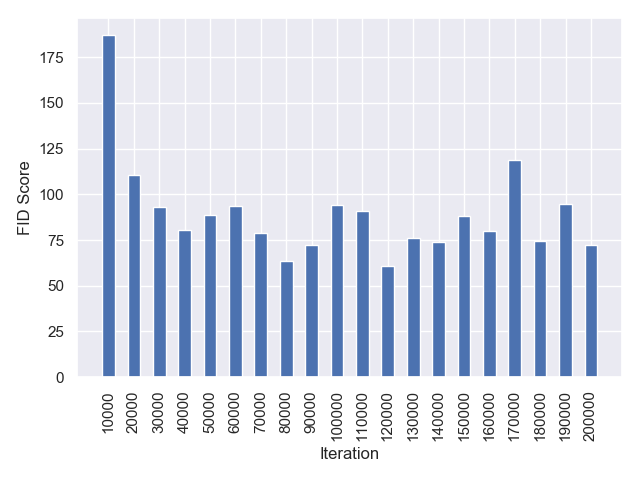
\includegraphics[width=0.47\linewidth]{figures/fid_plots/fid_score_cifar10.png}}
    \subfloat[CelebA]{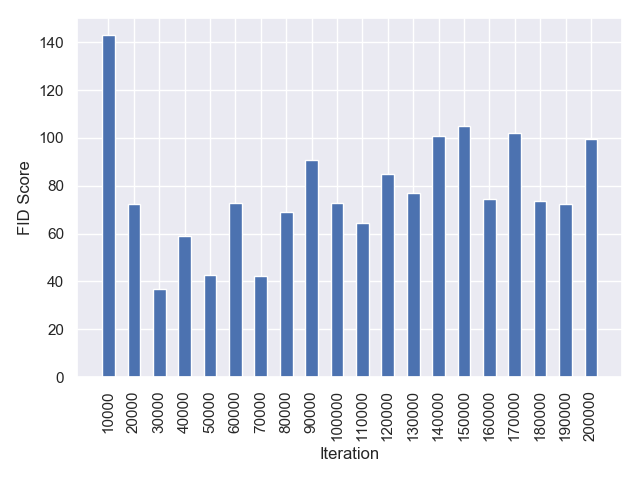
\includegraphics[width=0.47\linewidth]{figures/fid_plots/fid_score_celeb_a.png}}
    \caption{FID scores on 1000 samples for the model trained up to given iteration}
    \label{fig:fid}
\end{figure}

\vspace{1cm}

\begin{table}[h!]
    \centering
    \begin{tabular}{l c c c}
    \toprule
         & \multicolumn{3}{c}{Dataset} \\ \cmidrule{2-4}
         & MNIST & CIFAR-10 & CelebA \\ \midrule     
    Downloading data (required once) & 28.7s & 50.4s & 715.4s \\
    Training with RefineNet & 2.35it/sec & 1.73it/sec & 1.73it/sec \\
    Sampling (1 image) & 19s & 23s & 23s \\
    Sampling (100 images) & 112s & 158s & 158s \\
    Sampling (1000 images) & 910s & 1398s & 1398s \\ \bottomrule
    \end{tabular}
    \vspace{3mm}
    \caption{Time required for different components of the main experiment for each dataset. MNIST was run on a P100 GPU, while the other two datasets were run on a V100 GPU.}
    \label{tab:times}
\end{table}


\begin{figure}[h!]
    \centering
    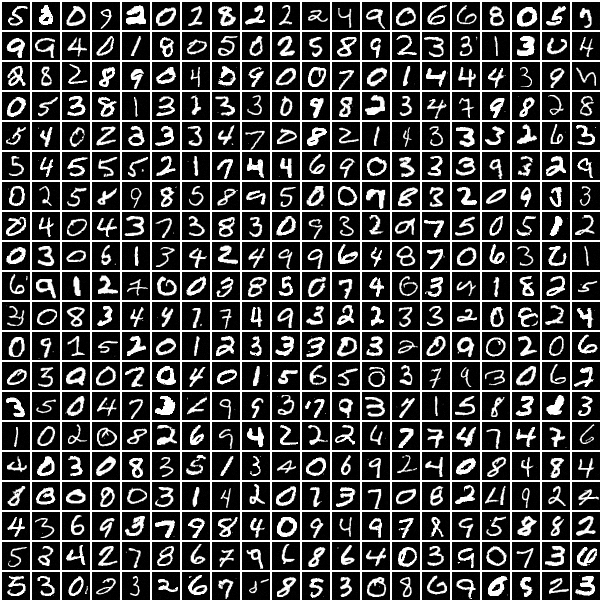
\includegraphics[width=\linewidth]{figures/samples/mnist_samples_large.png}
    \caption{Extended samples from MNIST}
    \label{fig:mnist-samples-large}
\end{figure}

\begin{figure}[h!]
    \centering
    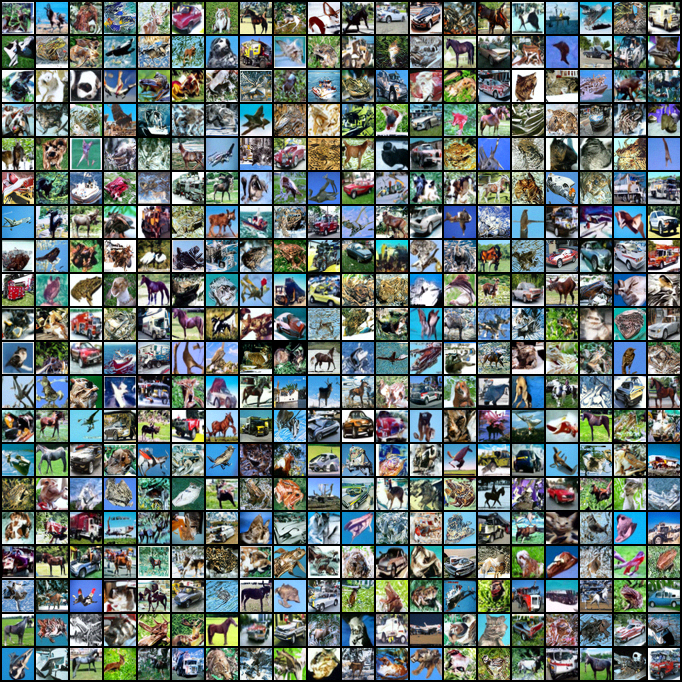
\includegraphics[width=\linewidth]{figures/samples/refinenet128_cifar10_L10_step120000_20x20.png}
    \caption{Extended samples from CIFAR10}
    \label{fig:cifar10-samples-large}
\end{figure}

\begin{figure}[h!]
    \centering
    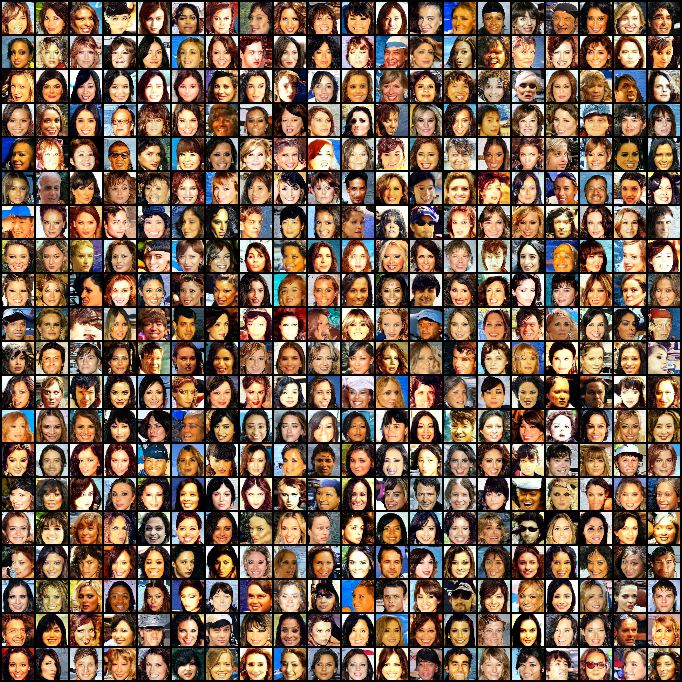
\includegraphics[width=\linewidth]{figures/samples/celeba_samples_large.png}
    \caption{Extended samples from CelebA}
    \label{fig:celeba-samples-large}
\end{figure}


\begin{figure}[h!]
  \centering
     \subfloat[MNIST]{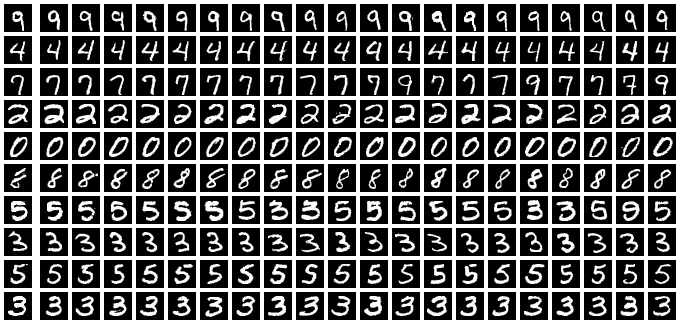
\includegraphics[width=0.91\linewidth]{figures/samples/refinenet64_mnist_L10_step200000_20nearest.png}\label{fig:mnist-nearest}}\\
     \subfloat[CIFAR-10]{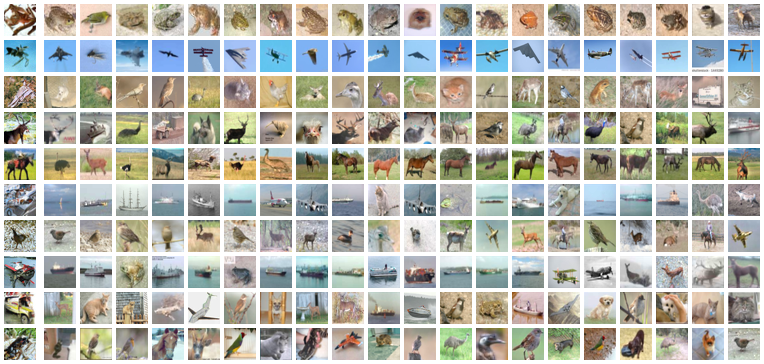
\includegraphics[width=0.9\linewidth]{figures/samples/refinenet128_cifar10_L10_step120000_20nearest.png}\label{fig:cifar10-nearest}}\\
     \subfloat[CelebA]{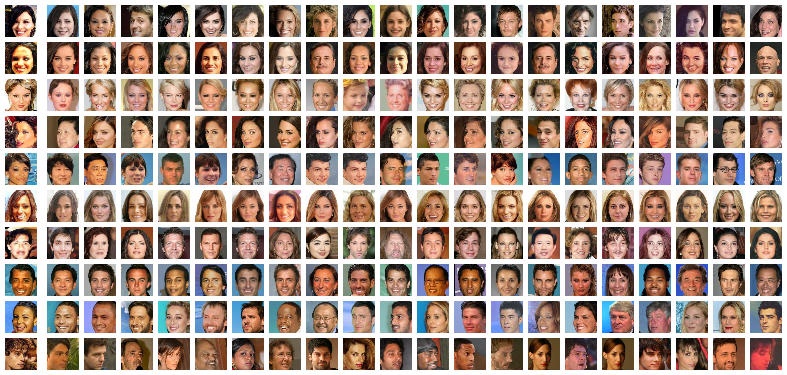
\includegraphics[width=0.9\linewidth]{figures/samples/refinenet128_celeb_a_L10_step30000_20nearest.png}\label{fig:celeba-nearest}}
     \caption{Samples (leftmost column) and their nearest neighbours from training set w.r.t. $l_2$ distance.}
     \label{fig:nn-large}
\end{figure}

\begin{figure}
    \centering
     \subfloat{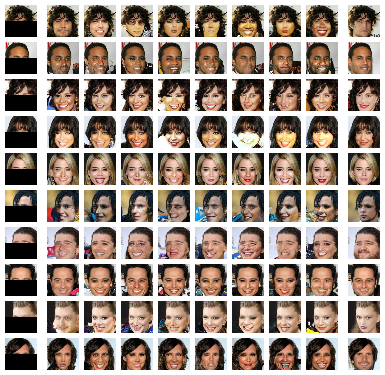
\includegraphics[width=0.75\linewidth]{figures/samples/refinenet128_celeb_a_L10_step30000_inpainting_occluded_down.png}\label{fig:celeb_a-inpaint_down}}\\
     \subfloat{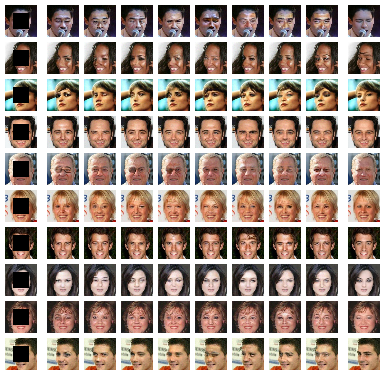
\includegraphics[width=0.75\linewidth]{figures/samples/other_occlusions/refinenet128_celeb_a_L10_step30000_inpainting_centered.png}\label{fig:celeb_a-inpaint_centered}}\\
     \caption{Recontruction with two more different patterns of occlusions on CelebA. Note that unlike the left-right occlusions shown in the main results, utilising face symmetry is not possible with these occlusions, once again proving the method has a good generative capacity.}
    \label{fig:celeb_a_inpainting}
\end{figure}